\documentclass[]{article}
\usepackage{cite}
\usepackage{lmodern}
\usepackage{amssymb,amsmath}
\usepackage{ifxetex,ifluatex}
\usepackage{fixltx2e} % provides \textsubscript
\ifnum 0\ifxetex 1\fi\ifluatex 1\fi=0 % if pdftex
  \usepackage[T1]{fontenc}
  \usepackage[utf8]{inputenc}
\else % if luatex or xelatex
  \ifxetex
    \usepackage{mathspec}
    \usepackage{xltxtra,xunicode}
  \else
    \usepackage{fontspec}
  \fi
  \defaultfontfeatures{Mapping=tex-text,Scale=MatchLowercase}
  \newcommand{\euro}{€}
\fi
% use upquote if available, for straight quotes in verbatim environments
\IfFileExists{upquote.sty}{\usepackage{upquote}}{}
% use microtype if available
\IfFileExists{microtype.sty}{%
\usepackage{microtype}
\UseMicrotypeSet[protrusion]{basicmath} % disable protrusion for tt fonts
}{}
\ifxetex
  \usepackage[setpagesize=false, % page size defined by xetex
              unicode=false, % unicode breaks when used with xetex
              xetex]{hyperref}
\else
  \usepackage[unicode=true]{hyperref}
\fi
\hypersetup{breaklinks=true,
            bookmarks=true,
            pdfauthor={},
            pdftitle={Linear Algebra},
            colorlinks=true,
            citecolor=blue,
            urlcolor=blue,
            linkcolor=magenta,
            pdfborder={0 0 0}}
\urlstyle{same}  % don't use monospace font for urls
\setlength{\parindent}{0pt}
\setlength{\parskip}{6pt plus 2pt minus 1pt}
\setlength{\emergencystretch}{3em}  % prevent overfull lines
\setcounter{secnumdepth}{0}

\newcommand{\argmax}[1]{\underset{#1}{\operatorname{argmax}}\; }
\newcommand{\argmin}[1]{\underset{#1}{\operatorname{argmin}}}
\newcommand{\spn}[1]{\operatorname{span}(#1)}


\usepackage{amsthm}
\theoremstyle{plain}
\newtheorem{thm}{Theorem}
\newtheorem{lem}[thm]{Lemma}
\newtheorem{prop}[thm]{Proposition}
\newtheorem*{cor}{Corollary}

\theoremstyle{definition}
\newtheorem{defn}{Definition}
\newtheorem{property}{Property}
\newtheorem{conj}{Conjecture}
\newtheorem{exmp}{Example}
\newtheorem*{exmp*}{Example}

\theoremstyle{remark}
\newtheorem*{rem}{Remark}
\newtheorem*{note}{Note}

\newcommand{\reals}{\mathbf{R}}
\newcommand{\ints}{\mathbf{Z}}
\newcommand{\rationals}{\mathbf{Q}}
\newcommand{\complex}{\mathbf{C}}

\usepackage{mathtools}
\newcommand\SetSymbol[1][]{\nonscript\:#1\vert\allowbreak\nonscript\:\mathopen{}}
\providecommand\given{} % to make it exist
\DeclarePairedDelimiterX\Set[1]\{\}{\renewcommand\given{\SetSymbol[\delimsize]}#1}

\newcommand{\smallcirc}{\mathbin{\text{\raisebox{0.2ex}{\scalebox{0.6}{$\circ$}}}}}

\newcommand\norm[1]{\left\lVert#1\right\rVert}
\newcommand\rank[1]{\operatorname{rank}\left( #1\right)}


\title{Stat 159/259: Linear Algebra Notes}
\author{Jarrod Millman}

\begin{document}
\maketitle

\begin{abstract}

These notes assume you've taken a semester of undergraduate linear algebra. In
particular, I assume you are familiar with the following:

\begin{itemize}
\itemsep1pt\parskip0pt\parsep0pt
\item solving systems of linear equations using Gaussian elimination
\item linear combinations of vectors to produce a space
\item the rank of a matrix
\item the Gram–Schmidt process for orthonormalising a set of vectors
\item eigenvectors and eigenvalues of a square matrix 
\end{itemize}

I will briefly review some of the above topics, but if you haven't seen them
before the presentation may be difficult to follow.  If so, please review your
introductory linear algebra textbook or use Wikipedia.

\end{abstract}

\section{Background}\label{background}

Introductory linear algebra texts often start with an examination of
simultaneous systems of linear equations.  For example, consider
the following system of linear equations
\begin{align*}
2x_1 + x_2 &= 3 \\
x_1 - 3x_2 &= -2.
\end{align*}

For convenience, we abbreviate this system

\begin{align*}
\underbrace{\begin{bmatrix} 2 & 1 \\ 1 & -3 \end{bmatrix}}_A \underbrace{\begin{bmatrix}x_1 \\ x_2\end{bmatrix}}_x
  &= \underbrace{\begin{bmatrix} 3 \\ -2\end{bmatrix}}_b
\end{align*}

where $A$ is the coefficient matrix, $x$ is a column vector of
unknowns, and $b$ is a column vector of constants.

You should verify that

\begin{align*}
x &= \begin{bmatrix}1 \\ 1\end{bmatrix}
\end{align*}

solves the given system.

More generally, a real-valued matrix $A$ is an ordered, $m \times n$ rectangular
array of real numbers, which when multiplied on the right by an $n$-dimensional
column vector $x$ produces an $m$-dimensional column vector
$b$.  Having introduced the $Ax = b$ notation, we
can view the $m \times n$ matrix $A$ as a linear function from $\reals^n$ to
$\reals^m$.  A linear function is one that respects proportions and for which
the effect of a sum is the sum of individual effects.  That is for any real
numbers $a$ and $b$ and any $n$-dimensional real vectors $x$ and
$y$, a function $A : \reals^n \to \reals^m$ is called a \emph{linear
function} if the following identity holds
\begin{align*}
A(ax + by) &= aA(x) + bA(y).
\end{align*}
Linear functions preserve linear combinations. 

Before returning our attention to real-valued matrices, let's remove some
detail to see what the basic objects of linear algebra are in an abstract
setting.

\section{Vector spaces and linear transforms}\label{vector-spaces-and-linear-transforms}

Linear algebra is the study of linear transformations of vector spaces over
some field.  To make this precise, we need to define a few algebraic
structures.

\begin{defn}
A \emph{group} $(G, \cdot)$ is a set $G$ and a binary operation $\cdot: G \times G \to G$
called (group) \emph{multiplication} such that
\begin{enumerate}
\item for all $a$ and $b$ in $G$, $ab$ is in $G$ (i.e., $G$ is \emph{closed} under multiplication),
\item for all $a, b,$ and $c$ in $G$, $(ab)c = a(bc)$ (i.e., multiplication is \emph{associative}),
\item there exists an \emph{identity} element $e$ in $G$ such that $eg = ge = g$ for all $g$ in $G$, and
\item for each $g$ in $G$ there exists an \emph{inverse} element $g^{-1}$ in $G$ such that $g^{-1}g = gg^{-1} = e$.
\end{enumerate}
\end{defn}

If the group multiplication is \emph{commutative} (i.e., $ab = ba$) then we say
the group is a \emph{commutative group}.  Given a group $(G, \cdot)$, a subset
$H$ of $G$ is called a \emph{subgroup} if $(H, \cdot)$ is a group under the
multiplication of $G$.

\begin{exmp*}
The integers under addition $(\ints, +)$ is a group with identity element $0$
and where the inverse of $z$ is $-z$.  The even integers are a subgroup of
$(\ints, +)$.  The rational numbers excluding $0$ under multiplication
$(\rationals\setminus \Set{0}, \cdot)$ is a group with identity element $1$ and
where the inverse of $p/q$ is $q/p$. In both cases, the reader should verify
that the group properties are met.
\end{exmp*}

\begin{defn}
A \emph{field} $(F, \times, +)$ is a set $F$ and two binary operations
called \emph{field multiplication} $\times: F \times F \to F$ and
\emph{field addition} $+: F \times F \to F$ such that $(F, +)$
is a commutative group with identity $0$ and $(F\setminus\{0\}, \times)$ is
a commutative group with identity denoted $1$ such that 
multiplication distributes over addition $a(b + c) = ab + ac$.
\end{defn}

We will mostly be interested in the field of real numbers $\reals$ and the
field of complex numbers $\complex$. However, note that the rationals
$\rationals$ equipped with the standard operations of addition and
multiplication form a field, while the integers $\ints$ do not (Why?).

\begin{defn}
A \emph{vector space} $(V, F, \oplus, \otimes)$ is set $V$ of \emph{vectors} over
a field $F$ of \emph{scalars} with the usual field operations equipped
with \emph{vector addition} $\oplus$ and \emph{scalar multiplication} $\otimes$ such
that $(V, \oplus)$ is a commutative group and scalar multiplication
$\otimes : F \times V \to V$ satisfies the following identities:
\begin{align*}
a\otimes(v  \oplus w) &= (a\otimes v)  \oplus (a\otimes w),  & 1\otimes v &= v, \\
(a + b)\otimes v &= (a\otimes v)  \oplus (b\otimes v), & (ab)\otimes v &= a\otimes (b\otimes v)
\end{align*}
for all vectors $v$ and $w$ in $V$ and all scalars $a$ and $b$ in $F$.
\end{defn}

While I used the symbols $\oplus$ and $\otimes$ in the definition above to
distinguish vector addition from field addition and scalar multiplication from
field multiplication, in the sequel I will follow standard practice and
overload the multiplication and addition symbols.  The type of multiplication
and addition will be made clear from the context.

The two operations of vector addition and scalar multiplication lead to the
more general notion of \emph{linear combinations} such as
\begin{align*}
a_1v_1 + a_2v_2 + \dots + a_nv_n = \sum a_iv_i
\end{align*}
of $n$ vectors $v_i$ in $V$ and $n$ scalars $a_i$ in $F$.
All linear combinations of a set of $n$ vectors $v_1, v_2, \dots, v_n$ of $V$
form a \emph{subspace} of $V$ \emph{spanned} by $v_1, v_2, \dots, v_n$.  A set
of $n$ vectors $v_1, v_2, \dots, v_n$ of $V$ are \emph{linearly independent} if
$\sum a_iv_i = 0$ implies that each $a_i$ is $0$.  A set of $n$ vectors
$v_1, v_2, \dots, v_n$ of $V$ form a \emph{basis} of a (finite-dimensional)
vector space when every vector in $V$ is uniquely expressed as a linear
combination of $v_1, v_2, \dots, v_n$.

\begin{defn}
Given two vector spaces $V$ and $W$ over the same field $F$, a function
$T : V \to W$ is called a \emph{linear transform} if for all vectors
$x$ and $y$ in $V$ and all scalars $a$ and $b$ in $F$
\begin{align*}
T(ax + bv) = aT(x) + bT(y).
\end{align*}
\end{defn}

While the focus of linear algebra concerns linear transformations of
vector spaces, we will often want to impose additional structure of
our vector spaces.  In particular, we would like to equip our spaces
with some notion of distance and angle.

\begin{defn}
Let $V$ be a vector space over the field $F$ with the usual operations.
Then an \emph{inner product} is any function
\begin{align*} 
\langle\cdot,\cdot\rangle : V \times V \to F
\end{align*}
which for all $x$, $y$,
and $z$ in $V$ and all $a$ and $b$ in $F$ the following hold
\begin{itemize}
\item \textbf{(Symmetry)} $\langle x, y\rangle = \langle y, x\rangle$,
\item \textbf{(Positive definite)} $\langle x, x\rangle \ge 0$ and $\langle x, x\rangle = 0$ implies $x=0$, and
\item \textbf{(Left linearity)} $\langle ax +by, z\rangle = a\langle x, z\rangle + b\langle y, z\rangle$.
\end{itemize}
\end{defn}

\begin{exmp*}
If $x$ is in $\reals^n$, then the dot product is an inner product. That is,
\begin{align*}
\langle x, y\rangle &= x^\top y = \sum x_i y_i = x_1 y_1 + x_2 y_2 + \dots + x_n y_n.
\end{align*}
You should verify that the dot product satisfies the properties for an
inner product.
\end{exmp*}

A vector space equipped with an inner product is called an \emph{inner product
space}.  Once we have an inner product we can define what we mean by distance
and angle.  Thus equipping the purely algebraic structure of a vector space
with an inner product enables us to rigorously define several geometric ideas
such as the length of a vector or the angle between two vectors.  Once we can
define the angle between vectors we will be able to establish a notion of
orthogonality (i.e., when are two vectors ``perpendicular'').  Inner product
spaces are an abstraction of Euclidean space, as inner products are an
abstraction of dot products.

\begin{defn}
Let $V$ be a vector space over a field $F$ equipped with an inner product.
Then any two vectors $x$ and $y$ are said to be \emph{orthogonal}, denoted
$x \perp y$, if their inner product is $0$.
\end{defn}

Two subspaces $U$ and $W$ of $V$ are called orthogonal if every vector in
$U$ is orthogonal to every vector in $W$.

\begin{defn}
Let $V$ be a vector space over a field $F$ equipped with an inner product
and let $W$ be any subspace of $V$.  The
\emph{orthogonal complement} of $W$ in $V$, denoted $W^\perp$, is the set
of all vectors in $V$ orthogonal to all vectors in $w$; that is,
\begin{align*}
W^\perp \equiv \Set{x \in V : x \perp w \text{ for all } w \in W}.
\end{align*}
\end{defn}

\begin{thm}[Orthogonal decomposition]
Let $V$ be a vector space over a field $F$ equipped with an inner product
and let $W$ be any subspace of $V$. Then
any vector $x$ in $V$ can be uniquely written as the sum of one element
from $W$ and one element from $W^\perp$.
\end{thm}
\begin{proof}
Clearly $W \cap W^\perp = \Set{0}$. Put $U = W + W^\perp$ (the space of
vectors obtained by adding all possible pairs chosen one from $W$ and
one from $W^\perp$). (Check that this is a subspace of $V$.)  Now take
an orthonormal basis for $U$. To show that $U = V$, assume not for a
contradiction.  If $U \ne V$, then extend the orthonormal basis for
$U$ to an orthonormal basis for $V$.  Let $z$ be one of the new basis
vectors in the extension.  Then $z \perp U$ by construction.  Since
$W \subset U$, $z \perp W$ as well.  But then $z$ must be an element
of $W^\perp$, a contradiction.  Hence $U = W + W^\perp = V$.  To show
that there is a unique representation, assume not for a contradiction.
If not, then there must be an $x$ in $V$ such that there are two
distinct, non-zero vectors $w_1 \ne w_2$ in $W$ and two 
distinct, non-zero vectors $u_1 \ne u_2$ in $W^\perp$ such that
$x = w_1 + u_1$ and $x = w_2 + u_2$.  This implies that
$(w_1 - w_2) + (u_1 - u_2) = 0$, a contradiction.
\end{proof}

\begin{cor}
Let $V$ be a vector space over a field $F$ equipped with an inner product
and let $W$ be any subspace of $V$. Then
\begin{align*}
\dim{V} = \dim{W} + \dim{W^\perp}.
\end{align*}
\end{cor}

\begin{defn}
Let $V$ be a vector space over a subfield $F$ of the complex numbers with the
usual operations.  Then a function
\begin{align*} 
\|\cdot\| : V \to \reals
\end{align*}
is called a
\emph{norm} on $V$ if for every $x$ and $y$ in $V$ and all $a$ in $F$ the
following properties hold
\begin{itemize}
\item \textbf{(Positivity)} $\|x\| \ge 0$;  and $\|x\| = 0$ implies $x=0$,
\item \textbf{(Absolute homogeneity)} $\|ax\| = |a|\|x\|$, and
\item \textbf{(Triangle inequality)} $\|x + y\| \le \|x\| + \|y\|$.
\end{itemize}
\end{defn}

\begin{note}
This definition is less general than the previous ones.  This is due
to the desire for the range of a norm to be a totally ordered field
(e.g., $\reals$ is totally ordered, but $\complex$ is not).
\end{note}

Given an inner product $\langle\cdot,\cdot\rangle$, there is a natural norm
for the space defined by that inner product
\begin{align*}
\|x\| \equiv \sqrt{\langle x, x\rangle}.
\end{align*}
If the inner product is the dot product, this is the usual Euclidean norm
\begin{align*}
\|x\| \equiv \sqrt{x^\top x}.
\end{align*}


\section{Matrices}\label{matrices}

There are four fundamental subspaces associated with any real-valued
$m \times n$ matrix $A$. Its \emph{nullspace} $N(A)$ contains all the vectors
$x$ that satisfy $Ax=0$.  Its \emph{column space} $R(A)$ is the set of all
linear combinations of its columns. The \emph{row space} of $A$ is the column
space $R(A^\top)$. Similarly, the \emph{left nullspace} is the nullspace
$N(A^\top)$.

The properties of the four fundamental subspaces are collected in the
fundamental theorem of the field.

\begin{thm}[The fundamental theorem of linear algebra]
Let $A$ be a $m \times n$ real-valued matrix with rank $r$.  Then
\begin{itemize}
\item $\dim R(A^\top) = \dim R(A) = r$
\item $\dim N(A^\top) = m - r$
\item $\dim N(A) = n - r$
\end{itemize}
and
\begin{itemize}
\item $R(A^\top) \perp N(A), \quad R(A^\top)^\perp = N(A), \quad N(A)^\perp = R(A^\top)$
\item $R(A) \perp N(A^\top), \quad R(A)^\perp = N(A^\top), \quad N(A^\top)^\perp = R(A)$
\end{itemize}
\end{thm}
\begin{proof}
That the row and column ranks are equal is usual shown in introductory courses
as a result of reducing $A$ to its row echelon form. Here is another approach.
Put $r \equiv \dim{R(A)}$ and let $u_1, u_2, \dots, u_r$ be a basis for the column
space of $A$.  Necessarily each column of $A$ is a unique linear combination of
this basis. Hence we can decompose $A$ as the product of two matrices $U$ and
$W$ where the columns of $U$ are the basis vectors for the column space of $A$
and the columns of $W$ are the unique coefficients (or weights) needed to combine
the basis vectors to produce the corresponding columns of $A$.
\begin{align*}
A &= \underbrace{\begin{bmatrix} | & & | \\
  u_1 & \cdots & u_r   \\
  | &  & | \\ 
\end{bmatrix}}_{U_{m \times r}}
\underbrace{\begin{bmatrix} | & & | \\
  w_1 & \cdots & w_n  \\
  | &  & | \\ 
\end{bmatrix}}_{W_{r \times n}}
 = \begin{bmatrix} | & & | \\
  Uw_1  & \cdots & Uw_n \\
  | &  & | \\ 
\end{bmatrix}
\end{align*}
%Now consider where the rows of $A$ come from in this decomposition
%\begin{align*}
%A &= \underbrace{\begin{bmatrix} \text{--- }  u_{1\cdot} \text{ ---} \\
%    \vdots     \\
%  \text{--- }  u_{m\cdot}  \text{ ---}  \\ 
%\end{bmatrix}}_{U_{m \times r}}
%\underbrace{\begin{bmatrix} \text{--- } w_{1\cdot} \text{ ---} \\
%    \vdots     \\
%  \text{--- }  w_{r\cdot}  \text{ ---}  \\ 
%\end{bmatrix}}_{W_{r \times n}}
% = \begin{bmatrix} \text{--- } u_{1\cdot} W \text{ ---} \\
%    \vdots     \\
%  \text{--- }  u_{m\cdot} W  \text{ ---}  \\ 
%\end{bmatrix}
%\end{align*}
Furthermore, the rows of $A$ can be written as linear combinations of the $r$ rows
of $W$.  Thus a basis for the row space must not exceed the number of rows in
$W$.  Hence, I conclude $\dim{R(A)} \ge \dim{R(A^\top)}$.  Applying the same
reasoning to $A^\top$ yields $\dim{R(A)} \le \dim{R(A^\top)}$.  Combining these
two inequalities, I conclude the two dimensions must be equal.

The remaining dimensionality results follow from the earlier orthogonal decomposition
theorem once we've proven the orthogonality properties.

To prove the first orthogonality property, we first note that for any $n$-dimensional
vector $x$ in the nullspace of $A$, it must be that $Ax = 0$.  Since $Ax = 0$,
$x$ is orthogonal to each row of $A$.  Thus $x$ is orthogonal to every linear
combination of the rows of $A$.  The second orthogonality property follows from
the same argument applied to $A^\top$.
\end{proof}

The theorem is illustrated schematically in Figure~\ref{fig:fourspaces} and
will be made concrete during our discussion of the singular value decomposition.

\begin{figure}
  \begin{centering}
    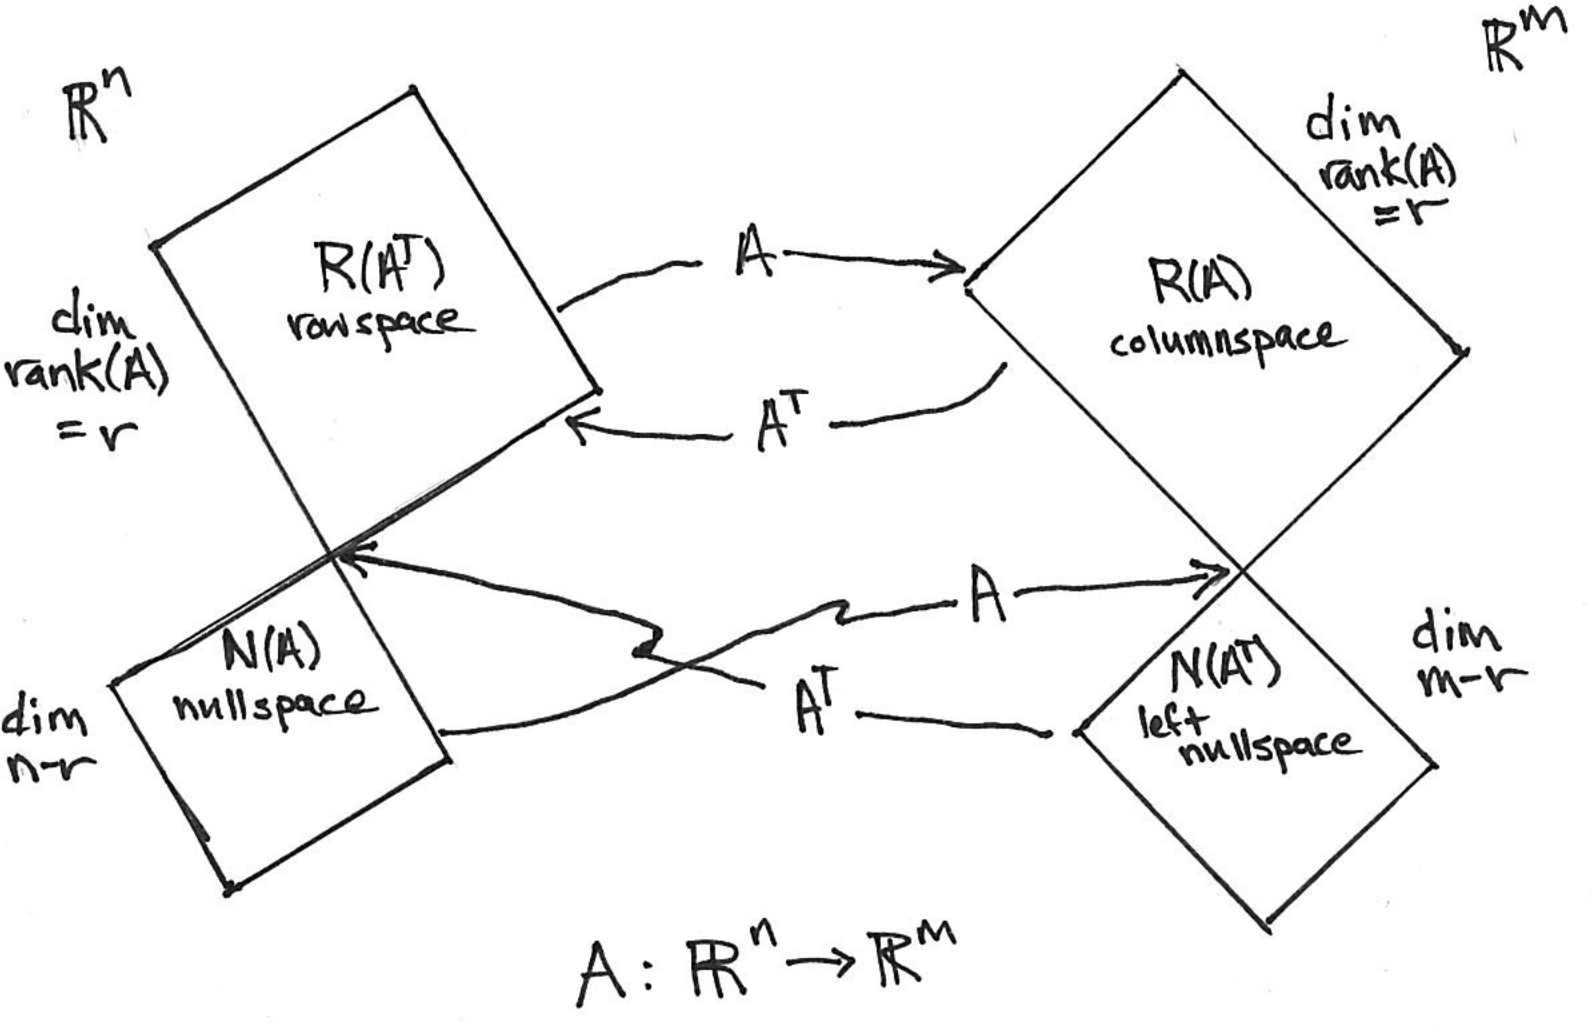
\includegraphics[width=4in]{fig/4-spaces.png}\par
  \end{centering}
  \caption{\label{fig:fourspaces}The four fundamental subspaces.}
\end{figure}

The fundamental theorem of linear algebra and the singular value decomposition
(SVD) are intimately related.  However, before discussing the SVD of an
arbitrary real-valued matrix, we will first consider certain nice matrices.
In particular, we will first look at (1) square matrices, then (2) square,
symmetric matrices, and finally (3) square, symmetric, positive (semi-)definite
matrices.  As we increasingly restrict our attention to more and more special
classes of matrices, our matrix decompositions will become nicer. Once we
derive the properties of the matrix decompositions of these restricted
matrices, we will use them to great effect when we return to the general case.

\subsection{Square matrices}\label{square-matrices}

A square matrix $A$ in $\reals^{n \times n}$ when multiplied on the right (or
left) by a vector $x$ in $\reals^n$ will produce another vector $y$ also in
$\reals^n$.  So it is possible that there may be directions in which $A$
behaves like a scalar.  That is there may be special vectors $v_i$ such that
$Av_i$ is just a scaled version of $v_i$.

\begin{defn}
Given $A$ in $\reals^{n \times n}$ a scalar $\lambda$ is called an
\emph{eigenvalue} and a vector $v$ its associated \emph{eigenvector} if
$Av = \lambda v$.
\end{defn}

If we had $n$ such eigenvalue-eigenvector pairs
$(\lambda_1, v_1), (\lambda_2, v_2), \dots, (\lambda_n, v_n)$,
then putting the $v_i$ in the columns of $S$ we can perform the following
calculation

\begin{align*}
 AS &= A \begin{bmatrix} | & & | \\
  v_1 & \cdots & v_n   \\
  | &  & | \\ 
\end{bmatrix} \\
&= \begin{bmatrix}
  | & & | \\
  Av_1 & \cdots & Av_n   \\
  | &  & | \\ 
\end{bmatrix}\\
&= \begin{bmatrix}
  | & & | \\
  \lambda_1 v_1 & \cdots & \lambda_n v_n   \\
  | &  & | \\ 
\end{bmatrix}\\
&=
\begin{bmatrix}
  | & & | \\
  v_1 & \cdots & v_n   \\
  | &  & | \\ 
\end{bmatrix}
\begin{bmatrix}\lambda_1\\
&  \ddots\\
&  & \lambda_n\end{bmatrix}\\
&= S\Lambda.
\end{align*}

Furthermore, if the eigenvectors are linearly independent then $S$ is full
rank, so its inverse $S^{-1}$ exists. Thus, we can \emph{diagonalize} $A$ by
\begin{align*}
S^{-1} A S &= \Lambda 
\end{align*}
or \emph{decompose} $A$ as
\begin{align*}
A &= S\Lambda S^{-1}.
\end{align*}

But how could we find them?  We can use Gaussian elimination to solve
$Ax = b$ for $x$ when $A$ and $b$ are given (that is, if $b$ is in the column
space of $A$).  But that will not work for solving $Ax = \lambda x$,
since we now have two unknowns $x$ and $\lambda$. However, notice that
if we move the RHS over to the LHS of the equation and pull $x$ outside
the sum, then
\begin{align*}
(A -  \lambda I)x &= 0.
\end{align*}

So if we hope to find a non-zero eigenvector $x$, then $(A -  \lambda I)$
will have to have a non-trivial null space. In other words, $(A -  \lambda I)$
must be singular.  Hence,
\begin{align*}
\det{(A -  \lambda I)} &= 0.
\end{align*}
Thus the roots of the $\det{(A -  \lambda I)}$ are the eigenvalues of $A$.
This function $\det{(A -  \lambda I)}$ is called the \emph{characteristic
polynomial} of $A$.  It is a $n$th degree polynomial in $\lambda$ and
by the fundamental theorem of algebra and the factor theorem it has
$n$ not necessarily distinct roots in the complex plane.

\subsection{Symmetric matrices}\label{symmetric-matrices}

A square matrix $A$ in $\reals^{n \times n}$ is \emph{symmetric} if
$A = A^\top$.

\begin{property}[$S^{-1} =  S^\top$]
If a symmetric matrix $A$ is full rank, then it is diagonalized by
$S^\top AS = \Lambda$ and decomposed as $A = S\Lambda S^\top$. 
\end{property}
\begin{proof}
By virtue of being a square matrix,
\begin{align*}
A = S\Lambda S^{-1}.
\end{align*}
Transposing both sides yields
\begin{align*}
A^\top = (S^{-1})^\top \Lambda S^\top.
\end{align*}
Since $A = A^\top$,
\begin{align*}
S\Lambda S^{-1} &=  (S^{-1})^\top \Lambda S^\top.
\end{align*}
I conclude $S^{-1} = S^\top$; and, since $A$ is square,
\textbf{Property 1} follows.
\end{proof}

\begin{property}[Real eigenvalues]
A symmetric, real-valued matrix $A$ has real eigenvalues.
\end{property}
\begin{proof}
Let $\lambda$ be an eigenvalue of $A$ and $v$ its associated eigenvector.
Then
\begin{align}\label{eq:p2a}
Av = \lambda v
\end{align}
implies
\begin{align}\label{eq:p2b}
A\overline{v} = \overline{\lambda} \overline{v}
\end{align}
where $\overline{v}$ is the complex conjugate of $v$.
Multiplying equation~\ref{eq:p2a} on the left by $\overline{v}^\top$ yields
\begin{align}\label{eq:p2c}
\overline{v}^\top Av = \lambda \overline{v}^\top v.
\end{align}
Transposing both sides of equation~\ref{eq:p2b} and replacing $A^\top$ with $A$ gives
\begin{align}\label{eq:p2d}
\overline{v}^\top A = \overline{\lambda} \overline{v}^\top.
\end{align}
Finally multiplying both sides of equation~\ref{eq:p2d} on the right by $v$ yields
\begin{align}\label{eq:p2e}
\overline{v}^\top Av  = \overline{\lambda} \overline{v}^\top v.
\end{align}
Since equation~\ref{eq:p2c} and equation~\ref{eq:p2e} have the same LHS,
\begin{align*}
\lambda \overline{v}^\top v = \overline{\lambda} \overline{v}^\top v.
\end{align*}
Canceling $\overline{v}^\top v$ from both sides, I conclude
$\lambda = \overline{\lambda}$.
\end{proof}

\begin{property}[Orthogonal eigenvectors]
For a symmetric, real-valued matrix $A$ with distinct eigenvalues
$\lambda_i \ne \lambda_j$, the associated eigenvectors are orthogonal
$v_i \perp v_j$.
\end{property}
\begin{proof}
Since $(Av_i)^\top = \lambda_i v_i^\top$, $A^\top = A$, and $Av_j = \lambda_j v_j$,
\begin{align*}
\lambda_i v_i^\top v_j &= v_i^\top A^\top v_j \\
   &= v_i^\top Av_j \\
   &= \lambda_j v_i^\top v_j.
\end{align*}
Subtracting the LHS from both sides of the above equation yields
\begin{align*}
(\lambda_i - \lambda_j) v_i^\top v_j &= 0.
\end{align*}
Since $(\lambda_i - \lambda_j) \ne 0$, I conclude $v_i^\top v_j = 0$.
\end{proof}

Let's summarize these nice properties in a theorem.

\begin{thm}[Spectral Theorem]
Let $A$ be a symmetric, real-valued $n \times n$ matrix. Then $A$ can be
decomposed as
\begin{align*}
A = Q\Lambda Q^\top
\end{align*}
where $Q$ is an orthogonal matrix (i.e., $Q^\top Q = I$) and $\Lambda$ is a
diagonal matrix containing the $n$ real eigenvalues, with multiplicity, of
$A$ sorted in non-increasing order
$\lambda_1 \ge \lambda_2 \ge \dots \ge \lambda_n$.
\end{thm}

I leave it as an exercise to show that for real symmetric matrices, you can
get orthogonal eigenvectors for repeated eigenvalues. The argument is straightforward,
but a bit cumbersome. 

\subsection{Positive (semi-)definite
matrices}\label{positive-semi-definite-matrices}

\begin{defn}
A symmetric, real-valued $n \times n$ matrix $A$ is \emph{positive
definite} if for all nonzero $x$ in $\reals^n$,
\begin{align*}
x^\top Ax > 0.
\end{align*}
\end{defn}

If we replace the strict inequality $>$ with $\ge$ above, then we say $A$
is \emph{positive semi-definite}.

\begin{thm}
A symmetric, real-valued, positive (semi-)definite matrix $A$ has (non-negative)
positive eigenvalues.
\end{thm}
\begin{proof}
Let $A = Q\Lambda Q^\top$ be the spectral decomposition of $A$ and let
$u_1, u_2, \dots, u_n$ be the eigenvectors of $A$ (i.e., the columns
of $Q$.  Since $A$ is symmetric, the eigenvectors are unitary $Q^\top Q = I$.
Hence, if we take $x$ to be $u_i$ for $i$ in $\{1, 2, \dots, n\}$,
\begin{align*}
u_i^\top Au_i &= u_i^\top Q\Lambda Q^\top u_i \\
  &= \lambda_i.
\end{align*}
Since $A$ is positive definite, I conclude $\lambda_i > 0$.  If $A$ is
positive semi-definite, then $\lambda_i \ge 0$.
\end{proof}

\begin{defn}
Let $A$ be a $m \times n$ matrix.  Then the $n \times n$ matrix $A^\top A$
is called the \emph{Gram matrix} of $A$.
\end{defn}

\begin{thm}
Let $A$ be any $m \times n$ matrix.  Then its Gram matrix $A^\top A$ is
positive semi-definite.
\end{thm}
\begin{proof}
For any $x$ in $\reals^n$,
\begin{align*}
x^\top A^\top Ax &= (Ax)^\top(Ax) \\
  &= \|Ax\|^2 \\
  &\ge 0.
\end{align*} 
\end{proof}

\begin{cor}
Let $A$ be any $m \times n$ matrix of rank $n$.  Then its Gram matrix
$A^\top A$ is positive definite.
\end{cor}

Note that we could have taken $A^\top$ instead of $A$ above, which would
lead to the Gram matrix $AA^\top$.



\subsection{Singular Value Decomposition}\label{svd}

We have seen that if $A$ has a particularly nice form (i.e., square
and symmetric), we can decompose it into the product of an
orthonormal basis, a diagonal matrix, and the transpose of the
first matrix.  Further, if $A$ is real-valued, then all the entries
of the matrix decomposition will also be real.  This decomposition
is particularly nice.  We can directly read off several properties
of $A$ by simply looking at its spectral decomposition.  For example,
the number of non-zero eigenvalues is the rank of $A$.

It would be extremely useful to be able to similarly decompose an arbitrary
real-valued $m \times n$ matrix $A$.  However, since we are now dealing with
a rectangular matrix, so the row space is a subspace of $\reals^m$ and
the column space is a subspace of $\reals^n$.  So rather than needing
just one orthonormal basis, we would like to decompose $A$ into an
orthonormal basis $V$ in the row space which goes to a scaled version
of an orthonormal basis $U$ for the column space
\begin{align*}
AV = U\Sigma
\end{align*}
where $V^\top V = I$, $U^\top U = I$, and $\Sigma$ is a diagonal matrix
of non-negative real numbers.

\begin{figure}
  \begin{centering}
    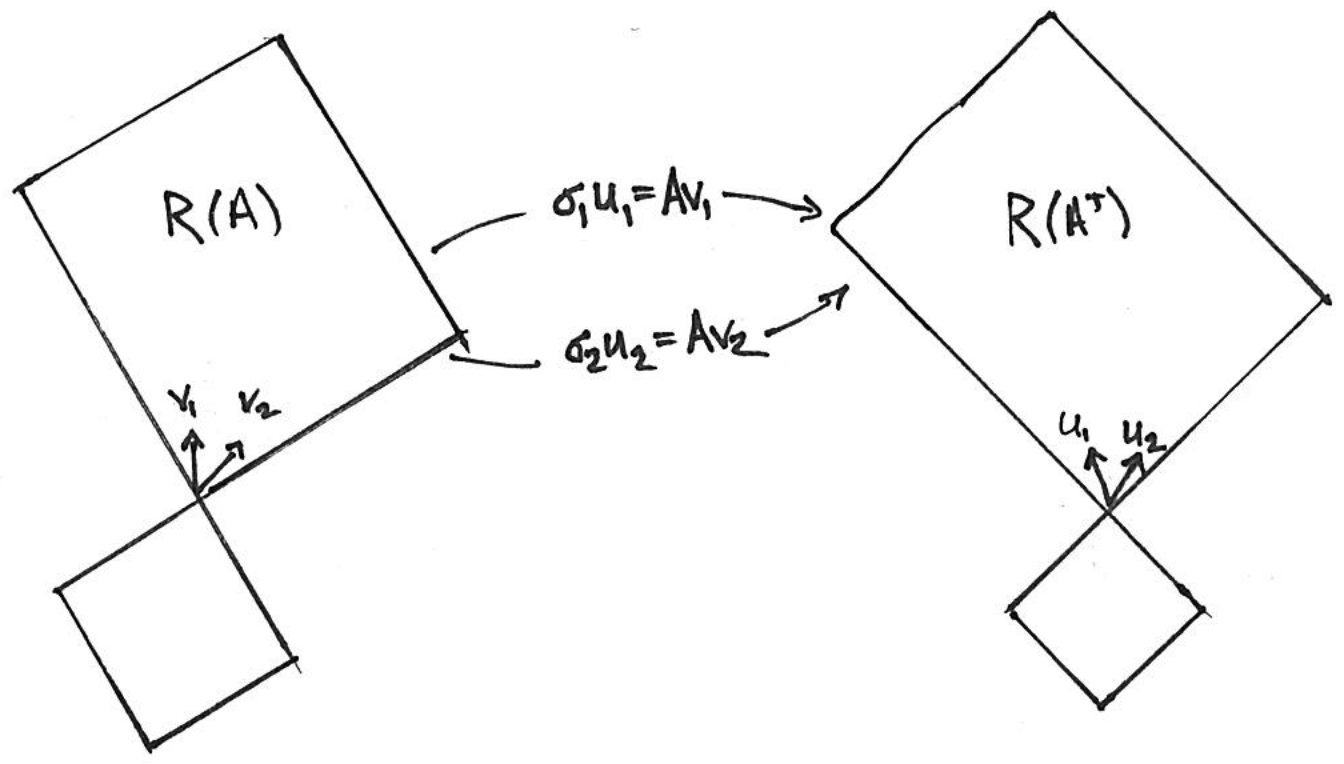
\includegraphics[width=5in]{fig/svd-hope.png}\par
  \end{centering}
  \caption{\label{fig:svd1}The goal.}
\end{figure}

See Figure~\ref{fig:svd1} and Figure~\ref{fig:svd2}.

\begin{thm}[Singular Value Decomposition]
Let $A$ be a real-valued $m \times n$ matrix.  Then its singular value
decomposition is $A = U \Sigma V^\top$.
\end{thm}
\begin{proof}
If $A = U \Sigma V^\top$, then
\begin{align*}
AA^\top &= (U \Sigma V^\top)(U \Sigma V^\top)^\top \\
    &= (U \Sigma V^\top)(V \Sigma U^\top) \\
    &= U \Sigma^2 U^\top
\end{align*}
and
\begin{align*}
A^\top A &= (U \Sigma V^\top)^\top (U \Sigma V^\top) \\
   &= (V \Sigma U^\top)  (U \Sigma V^\top) \\
   &= V \Sigma^2 V^\top.
\end{align*}
Hence if we could decompose $AA^\top = U \Sigma^2 U^\top$ and
$A^\top A = V \Sigma^2 V^\top$.
\end{proof}

\begin{figure}
  \begin{centering}
    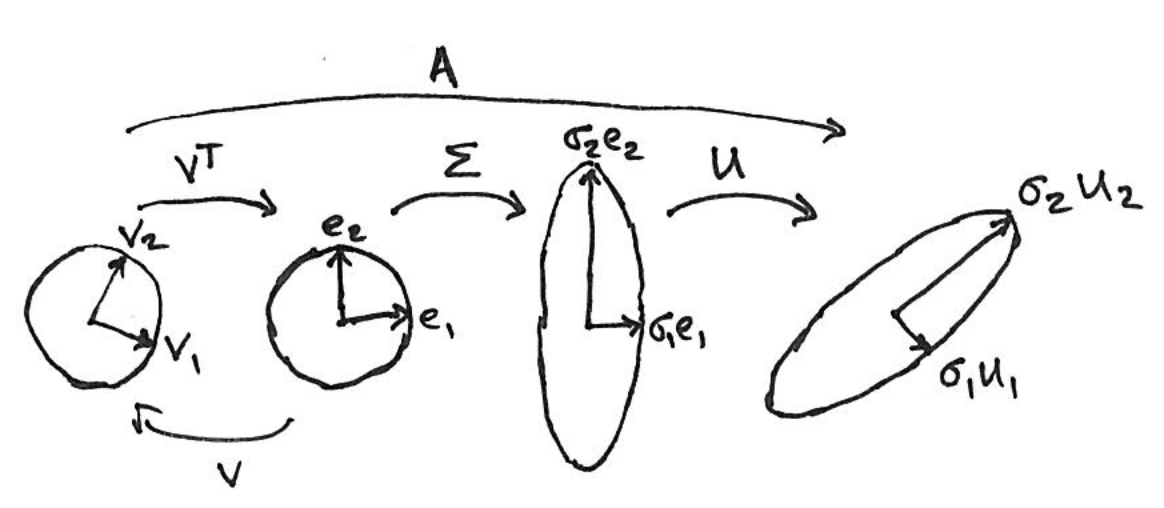
\includegraphics[width=5in]{fig/action-via-svd.png}\par
  \end{centering}
  \caption{\label{fig:svd2}The action of $A$ via its SVD.}
\end{figure}

\section{Variational characterization of
eigenvalues}\label{variational-characterization-of-eigenvalues}

\begin{defn}
For any square $n \times n$ matrix $A$ and any $n$-dimensional vector
$x$, the Rayleigh Quotient is
\begin{align*}
\frac{x^\top A x}{x^\top x}.
\end{align*}
\end{defn}

Note that if $x^\top x = 1$, this is equivalent to $x^\top A x$.

\begin{thm}[Rayleigh Quotient Theorem]
Let $A$ be a symmetric matrix in $\reals^{n \times n}$ and let
$A = Q\Lambda Q^\top$ be its spectral decomposition.  Since $A$
has real eigenvalues, let $\lambda_1 \ge \lambda_2 \ge \dots \ge \lambda_n$.
Then
\begin{align*}
\lambda_1 &= \max_{\|x\|=1} x^\top A x \\
\lambda_n &= \min_{\|x\|=1} x^\top A x
\end{align*}
\end{thm}
\begin{proof}
For any $\|x\|=1$ in $\reals^n$, put $y = Q^\top x$.  Note that there is
a one-to-one correspondence between $x$ and $y$.  By the rotational invariance
of the Euclidean norm, we have $\|y\| = \|Q^\top x\| = \|x\|= 1$. Hence
\begin{align*}
x^\top A x &= x^\top Q\Lambda Q^\top x \\
  &= y^\top \Lambda y \\
  &= \sum \lambda_i y_i^2.
\end{align*}
By assumption, $\lambda_1 \ge \lambda_i \ge \lambda_n$ for $i$ in
$\{1, 2, \dots, n\}$, so
\begin{align*}
\lambda_1 = \lambda_1 \sum y_i^2 \ge \sum \lambda_i y_i^2 \ge  \lambda_n \sum y_i^2 = \lambda_n.
\end{align*}
Since the inequalities are obtained with $v_1$ and $v_n$ respectively, we are
done.
\end{proof}

\begin{thm}[Poincair\'{e} Inequality]
Let $A$ be a symmetric matrix in $\reals^{n \times n}$ and let
$A = Q\Lambda Q^\top$ be its spectral decomposition.  Since $A$
has real eigenvalues, let $\lambda_1 \ge \lambda_2 \ge \dots \ge \lambda_n$.
Fix $k$ in $\{1, 2, \dots, n\}$.
Let $V$ denote any $k$-dimensional subspace of $\reals^n$.  Then
there exists $x$ and $y$ in $V$ such that
\begin{align*}
\lambda_k &\ge x^\top A x \\
\lambda_{n-k+1} &\le y^\top A y
\end{align*}
\end{thm}
\begin{proof}
Put
\begin{align*}
Q_k &=  \begin{bmatrix} | & & | \\
  v_k & \cdots & v_n   \\
  | &  & | \\ 
\end{bmatrix}.
\end{align*}
Let $W$ denote the column space of $Q_k$.  Clearly, the $\dim W = n-k+1$.  So
by a counting argument $V$ and $W$ have a non-trivial intersection.  For any
$\|x\|=1$ in $V \cap W$, there exists a $y$ in $\reals^{n-k+1}$ such that
$x = Q_k y$. Hence
\begin{align*}
x^\top A x &= y^\top Q_k^\top Q\Lambda Q^\top Q_k y \\
   &= \sum_{i=k}^n \lambda_i y_i^2 \\
   &\le \lambda_k.
\end{align*}
To show $\lambda_{n-k+1} \le y^\top A y$, apply the previous result
to $-A$.
\end{proof}

\begin{thm}[The Minimax Principle]
Let $A$ be a symmetric matrix in $\reals^{n \times n}$ and let
$A = Q\Lambda Q^\top$ be its spectral decomposition.  Since $A$
has real eigenvalues, let $\lambda_1 \ge \lambda_2 \ge \dots \ge \lambda_n$.
Fix $k$ in $\{1, 2, \dots, n\}$.
Let $V$ denote any subspace of $\reals^n$ (the dimension of which will be
specified below).  Then
\begin{align*}
\lambda_k &= \max_{\dim{V} = k} \quad \min_{\substack{x \in V \\ \|x\|=1}} \; x^\top A x \\
  &= \min_{\dim{V} = n-k+1} \quad \max_{\substack{x \in V \\ \|x\|=1}} \; x^\top A x.
\end{align*}
\end{thm}
\begin{proof}
By the Poincair\'{e} inequality, in any $k$-dimensional subspace $V$ of
$\reals^n$ there is an unit length vector $x$ such that
$\lambda_k \ge x^\top A x$.  Hence it is true that for any $k$-dimensional
subspace $V$
\begin{align*}
\lambda_k \ge \min_{\substack{x \in V \\ \|x\|=1}} x^\top A x.
\end{align*}
Since this bound is obtained by letting $x = v_k$, I conclude
\begin{align*}
\lambda_k &= \max_{\dim{V} = k} \quad \min_{\substack{x \in V \\ \|x\|=1}} \; x^\top A x.
\end{align*}
For the second result, apply the first result to $-A$.
\end{proof}

This is also known as the \emph{Variational theorem} or the
\emph{Courant-Fisher-Weyl minimax theorem}.

\section{Orthogonal projections}\label{projections}



\begin{defn}
An $n \times n$ matrix $P$ is an \emph{orthogonal projection} matrix
if $P=P^2$ and $P=P^\top$.
\end{defn}

\begin{thm}
Let $A$ be a real-valued matrix in $\reals^{m \times n}$ of rank $n$.
The matrix $P_A = A (A^\top A)^{-1} A^\top$ when multiplied on the
right by a vector $x$ in $\reals^n$ will return 
\end{thm}
\begin{proof}
The orthogonal projection $p$ of $v$ onto the column space of $A$, which has
full column rank, will be a unique combination of the columns of $A$; that is,
$p=Ax$ for some unknown $x$ in $\reals^n$.  Since it is an orthogonal
projection, the difference $e=v-p$ will be orthogonal to the column space of
$A$.  In particular, $e \perp A$; so
\begin{align*}
A^\top e =  A^\top(v-p) =  A^\top(v-Ax) =  A^\top v -  A^\top Ax = 0.
\end{align*}
Hence
\begin{align*}
A^\top Ax = A^\top v.
\end{align*}
Since $A$ has full column rank, $(A^\top A)^{-1}$ exists. So
\begin{align*}
x = (A^\top A)^{-1}A^\top v
\end{align*}
and
\begin{align*}
p = Ax = \underbrace{A(A^\top A)^{-1}A^\top}_{P_A} v.
\end{align*}
See Figure~\ref{fig:orthoprojection} for a schematic illustration.
\end{proof}
\begin{figure}
  \begin{centering}
    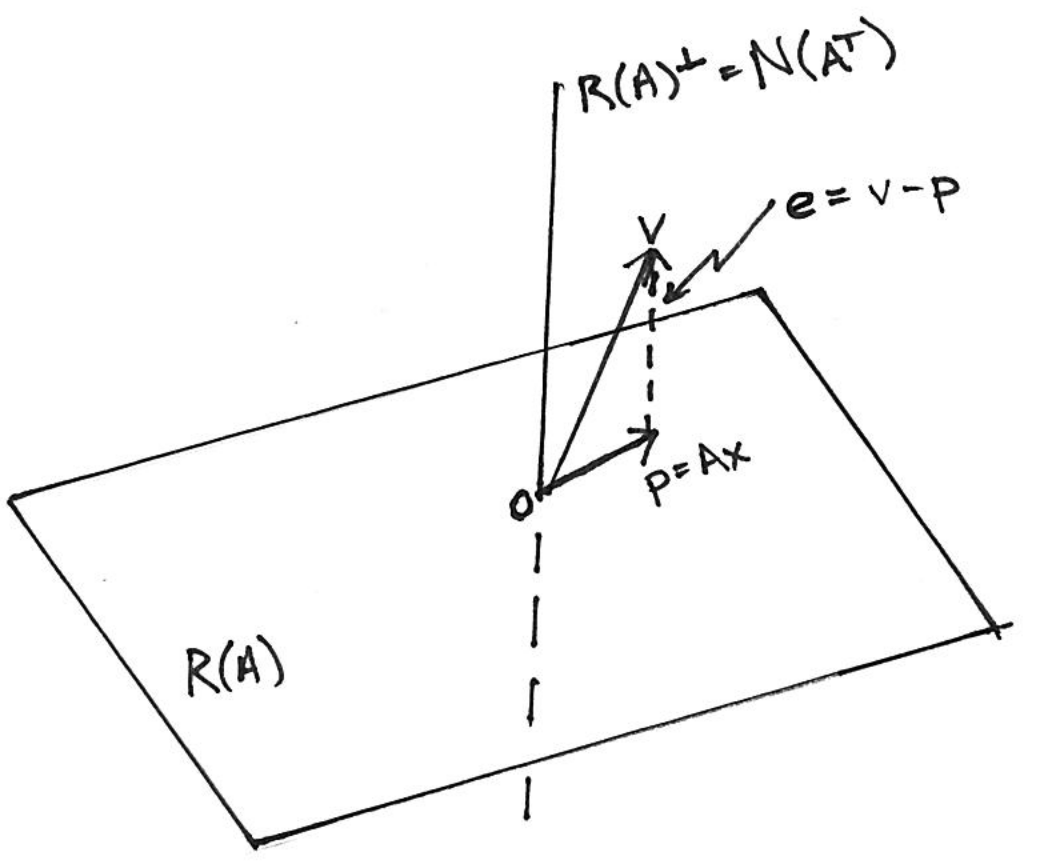
\includegraphics[width=3in]{fig/orthoproject.png}\par
  \end{centering}
  \caption{\label{fig:orthoprojection}Schematic illustration of orthogonal projection.}
\end{figure}


\section{Applications}\label{applications}

We are now ready to look at three important applications:  pseudoinverses,
principal component analysis, and the least square solution.

\subsection{Pseudoinverse}\label{pseudoinverse}

We begin by reviewing some facts about matrix inverses.

\begin{defn}
A matrix $A$ has a \emph{left inverse} $A_\text{L}^{-1}$ if $A_\text{L}^{-1}A=I$.
\end{defn}

If $A$ is full column rank, then it has a trivial null space and $A^\top A$ is
full rank.  Hence $(A^\top A)^{-1}$ exists and $(A^\top A)^{-1}A^\top A = I$.
In this case, we say $A_\text{L}^{-1} = (A^\top A)^{-1}A^\top$ is a left
inverse of $A$ (this doesn't mean that it is unique).

\begin{defn}
A matrix $A$ has a \emph{right inverse} $A_\text{R}^{-1}$ if $AA_\text{R}^{-1}=I$.
\end{defn}

Similarly, if $A$ is full row rank, then  $(AA^\top)^{-1}$ exists and
$AA^\top(A A^\top)^{-1} = I$. Then we say $A_\text{R}^{-1} = A^\top(A A^\top)^{-1}$
is a (not necessarily unique) right inverse of $A$.

\begin{defn}
If a matrix $A^{-1}$ is both a left and a right inverse of a matrix $A$, it is
called the \emph{inverse} of $A$.
\end{defn}

\begin{thm}
If a square matrix $A$ has a left inverse $A_\text{L}^{-1}$ and a right inverse
$A_\text{R}^{-1}$, then $A_\text{L}^{-1}=A_\text{R}^{-1}$.
\end{thm}
\begin{proof}
Since all the dimensions match,
\begin{align*}
A_\text{L}^{-1} &= A_\text{L}^{-1}AA_\text{R}^{-1} \\
  &= A_\text{R}^{-1}.
\end{align*}
\end{proof}

\begin{defn}
A real-valued matrix $A$ has a \emph{pseudoinverse} $A^+$ if
\begin{itemize}
\item $AA^+A = A$,
\item $A^+AA^+ = A^+$,
\item $(A^+A)^\top = A^+A$, and
\item $(AA^+)^\top = AA^+$.
\end{itemize}
\end{defn}

\begin{thm}[Existence and uniquness of $A^+$]
For any real-valued $m \times n$ matrix $A$ there is a unique pseudoinverse
$A^+$.
\end{thm}
\begin{proof}
By computing $A^+$ via SVD below, I demonstrate the existence of $A^+$
for any real-valued matrix $A$.  To show uniqueness, suppose both $A_1^+$ and
$A_2^+$ are pseudoinverses of $A$.  Then, by repeated application of the
properties of the pseudoinverse, I have
\begin{align*}
AA_1^+ &= (AA_1^+)^\top \\
 &= (A_1^+)^\top A^\top \\
 &= (A_1^+)^\top (AA_2^+A)^\top \\
 &= (A_1^+)^\top A^\top (A_2^+)^\top A^\top \\
 &= (AA_1^+)^\top (AA_2^+)^\top \\
 &= AA_1^+AA_2^+ \\
 &= AA_2^+.
\end{align*}
Similarly, $A_1^+A = A_2^+A$. Hence
\begin{align*}
A_1^+ = A_1^+AA_1^+ = A_2^+AA_1^+ = A_2^+AA_2^+ = A_2^+.
\end{align*}
\end{proof}

\begin{thm}[Computing $A^+$ via SVD]
For any real-valued matrix $A$, let $U\Sigma V^\top$ be its SVD. Then the
pseudoinverse of $A$ is
\begin{align*}
A^+ = V\Sigma^+U^\top,
\end{align*}
where $\Sigma^+$ is formed by transposing $\Sigma$ and replacing each non-zero
$\sigma_i$ with its reciprocal $1/\sigma_i$.
%\begin{align*}
%\Sigma^+ = \begin{bmatrix} \sigma_1^{-1} & & & & & \\
% & \ddots & & & &  \\
% & & \sigma_r^{-1} & & & \\
% & & & & & \\
% & & & & & \\
%\end{bmatrix} 
%\end{align*}
\end{thm}
\begin{proof}
Since $V^\top V = I$, $U^\top U = I$, and $\Sigma \Sigma^+ \Sigma = \Sigma$,
\begin{align*}
AA^+A &=  (U\Sigma V^\top) (V\Sigma^+U^\top) (U\Sigma V^\top) \\
 &= U\Sigma V^\top \\
 &= A.
\end{align*}
Similarly,
\begin{align*}
A^+AA^+ &= (V\Sigma^+U^\top) (U\Sigma V^\top)(V\Sigma^+U^\top) \\
  &= A^+.
\end{align*}
Since $\Sigma \Sigma^+ = \Sigma^+ \Sigma$,
\begin{align*}
(A^+A)^\top &= ( (V\Sigma^+U^\top) (U\Sigma V^\top) )^\top \\
  &= V\Sigma \Sigma^+ V^\top \\
  &= V\Sigma^+ \Sigma V^\top \\
  &= V\Sigma^+U^\top U\Sigma V^\top \\
  &= A^+A.
\end{align*}
Finally,
\begin{align*}
(AA^+)^\top &= ((U\Sigma V^\top) (V\Sigma^+U^\top) )^\top\\
 &= AA^+.
\end{align*}
I conclude that $A^+$ satisfies all the requirements of a pseudoinverse.
\end{proof}

\subsection{Principal Component Analysis}\label{pca}

\begin{defn}
The \emph{matrix of ones} is a matrix where every entry is $1$.  We will
denote an $n \times n$ matrix of ones as $J_n$.
\end{defn}

\begin{defn}
Given $n$ samples of an $m$-dimensional random vector,
\begin{align*}
X &= \begin{bmatrix} | & & | \\
  x_1 & \cdots & x_n   \\
  | &  & | \\ 
\end{bmatrix}
\end{align*}
the \emph{sample mean vector} is
\begin{align*}
\bar{x} = \frac{1}{n}\sum x_i
\end{align*}
and the \emph{sample covariance matrix} is
\begin{align*}
\hat{\Sigma} = \frac{1}{n-1}\sum (x_i - \bar{x})(x_i - \bar{x})^\top.
\end{align*}
\end{defn}

\begin{defn}
The \emph{centering matrix} of size $n$ is defined as
\begin{align*}
C_n &= I_n - \frac{1}{n}J_n,
\end{align*}
where $J_n$ is the $n \times n$ matrix of all $1$s.
\end{defn}

You should verify that the centering matrix $C_n$ is symmetric $C_n = C_n^\top$
and idempotent $C_n^2 = C_n$.  Given an $m \times n$ matrix $X$, multiplying it
with centering matrix on the left $C_m X$ removes the column mean from each
column. Similarly, multiplying $X$ with centering matrix on the right $XC_n$
removes the row mean from each row. While this is not computationally efficient,
it is convenient for algebraic manipulation (as we will see).

\begin{defn}
Given an $m \times n$ data matrix $X$, the \emph{scatter matrix} is the
$m \times m$ matrix
\begin{align*}
S &\equiv \sum (x_i - \bar{x})(x_i - \bar{x})^\top \\
 &= (X - \bar{x}\mathbf{1}^\top)  (X - \bar{x}\mathbf{1}^\top)^\top \\
 &= (XC_n)(XC_n)^\top \\
 &= XC_nC_n^\top X^\top \\
 &= XC_n X^\top.
\end{align*}
\end{defn}

Scaling the scatter matrix by $\frac{1}{n-1}$ yields the standard sample covariance matrix,
while scaling it by $\frac{1}{n}$ yields the maximum likelihood estimate of the covariance
matrix of the multivariate Gaussian distribution.

\subsubsection{SVD, revisited}

Since the SVD is so important, it is worth looking at it from a different
perspective.  Consider the following greedy strategy of search first for
the unit direction which $A$ increases most

\begin{align*}
v_1 &= \argmax{\|v\|=1} \|A v\| \\
\lambda_1 &= \|A v_1\|. \\
\end{align*}

Then the unit direction perpendicular to the first which $A$ increases most

\begin{align*}
v_2 &= \argmax{\substack{\|v\|=1 \\ v \perp v_1}} \|A v\| \\
\lambda_2 &= \|A v_2\| .
\end{align*}

And then the unit direction perpendicular to the space spanned by the first
two principle directions which $A$ increases most

\begin{align*}
v_3 &= \argmax{\substack{\|v\|=1 \\ v \perp v_1, v_2}} \|A v\| \\
\lambda_3 &= \|A v_3\| .
\end{align*}

And continuing in this way until there are no more unit direction perpendicular
to all the previous ones.

\begin{thm}[Best-fit linear subspace]
Let $A$ be a $m \times n$ matrix with right singular vectors $v_1, v_2, \dots, v_r$.
For $1\le k \le r$, let $V_k=\spn{v_1, v_2, \dots, v_k}$ be the space spanned
by the first $k$ right singular values of $A$.  Then $V_k$ is the best-fit
$k$-dimensional subspace for $A$.
\end{thm}
%\begin{proof}
%\end{proof}

\begin{defn}
For any real matrix $A$ with the SVD given as $U\Sigma V^\top$, the \emph{truncated
SVD} of $A$ is $A_k = U\Sigma_k V^\top$ where $\Sigma_k$ is obtained from
$\Sigma$ by setting all but the first $k<\rank{A}$ elements of the diagonal to $0$.
\end{defn}

Note that all but the first $k$ columns of $U$ and all but the first $k$ rows of
$V^\top$ will be multiplied by $0$, so $U\Sigma_k V^\top$ is equivalent to
$U_k\Sigma_k V_k^\top$ where $U_k$ is just the first $t$ columns of $U$ and
$V_k^\top$ is just the first $k$ rows of $V^\top$.

\begin{cor}[Eckart–Young theorem]
The truncated SVD $A_k$ is the best rank $k$ approximation to $A$ in the sense that
if $B$ is any compatible rank $k$, then
\begin{align*}
\norm{A - A_k}_F \le \norm{A - B}_F.
\end{align*}
\end{cor}
%\begin{proof}
%For any matrix $M$, the Frobenius norm $\norm{M}_F$ of $M$ is the sum of the
%Euclidean norms of its columns.
%\end{proof}

\subsection{Least squares solution}\label{least-squares-solution}

Consider the least-squares problem
\begin{align*}
p^\ast &= \min_x \|Ax-y\|_2
\end{align*}
for $A$ in $\reals^{m \times n}$ and $y$ in $\reals^m$.

If $y$ is in $R(A)$, then $p^\ast = 0$.  However, if $y$ is not in $R(A)$,
then $p^\ast > 0$ and, at optimum, the residual vector $r = y - Ax$ is such
that $r^\top y > 0, A^\top r = 0$.  I will assume
that $m \ge n$, and that $A$ is full column rank.

Using the SVD of $A$ and the rotational invariance of the $L_2$ norm,
\begin{align*}
\min_x \|Ax-y\|_2 &= \min_x \|Ax-y\|_2^2 \\
 &= \min_x \|U^\top(A VV^\top x-y)\|_2^2 \\
 &= \min_x \|\Sigma V^\top x-U^\top y)\|_2^2.
\end{align*}
Let
\begin{align*}
 \tilde{x} &\doteq V^\top x \quad \text{ and } \quad
 \tilde{y} \doteq U^\top y = \begin{bmatrix} u_1^\top y \\ \vdots \\ u_m^\top y  \\ u_{m+1}^\top y \\ \vdots\\ u_n^\top y\end{bmatrix}
  = \begin{bmatrix} \tilde{y}_{_{\mathcal{R}(A)}} \\ \tilde{y}_{_{\mathcal{R}(A)^\perp}} \end{bmatrix}
\end{align*}

where I've partitioned $\tilde{y}$ into the first $m$ elements
$\tilde{y}_{_{\mathcal{R}(A)}}$ and the remaining $n-m$ elements
$\tilde{y}_{_{\mathcal{R}(A)^\perp}}$.

Let $\tilde{\Sigma}$ denote the first $m$ rows of $\Sigma$, which by assumption
is the diagonal matrix of the $m$ singular values.  Substituting these symbols into the
above equation and expanding the sum into two terms (one containing $\tilde{x}$
and the other not), I have

\begin{align*}
\min_x \|\Sigma V^\top x-U^\top y)\|_2^2
  &= \min_{\tilde{x}} \norm{ \begin{bmatrix}\tilde{\Sigma} \\ 0 \end{bmatrix}\tilde{x} - \begin{bmatrix} \tilde{y}_{_{\mathcal{R}(A)}} \\ \tilde{y}_{_{\mathcal{R}(A)^\perp}}  \end{bmatrix}}_2^2 \\
  &= \min_{\tilde{x}} \norm{\begin{matrix} \tilde{\Sigma} \tilde{x} - \tilde{y}_{_{\mathcal{R}(A)}} \\ \tilde{y}_{_{\mathcal{R}(A)^\perp}}\end{matrix}}_2^2  \\
  &= \min_{\tilde{x}} \|\tilde{\Sigma}\tilde{x} -  \tilde{y}_{_{\mathcal{R}(A)}} \|_2^2 + \|\tilde{y}_{_{\mathcal{R}(A)^\perp}}\|_2^2.
\end{align*}

Since $\tilde{\Sigma}$ is invertible (just replace the non-zero elements with
their reciprocals), the first term can be made $0$ by setting
$\tilde{x} = \tilde{\Sigma}^{-1} \tilde{y}_{_{\mathcal{R}(A)}}$.  I conclude $p^\ast =  \|\tilde{y}_{_{\mathcal{R}(A)^\perp}}\|_2^2$ and
the least square solution is given by $\hat{x} = V^\top\tilde{\Sigma}^{-1} \tilde{y}_{_{\mathcal{R}(A)}}$.

By construction $\tilde{y}_{_{\mathcal{R}(A)^\perp}}$ is colinear with a component of $\tilde{y}$
and thus with $y$.  Hence $r^\top y > 0$.  Also by construction, $\tilde{y}_{_{\mathcal{R}(A)^\perp}}$
is perpendicular to $A$.  Hence $A^\top r = 0$.  The geometry is schematically illustrated in
Figure~\ref{fig:ls-geom}.
\begin{figure}
  \begin{centering}
    \includegraphics[width=3in]{fig/ls-geom.pdf}\par
  \end{centering}
  \caption{\label{fig:ls-geom}This diagram represents the geometry of least squares.}
\end{figure}


\nocite{*}
\bibliographystyle{plain}
\bibliography{linear-algebra}

\end{document}
